\documentclass{article}
\usepackage{tikz,xcolor,geometry}
\geometry{paperwidth=23.7cm,paperheight=6.2cm,left=0pt,right=0pt,top=2pt,bottom=0pt}
\pagestyle{empty}
\begin{document}
\centering
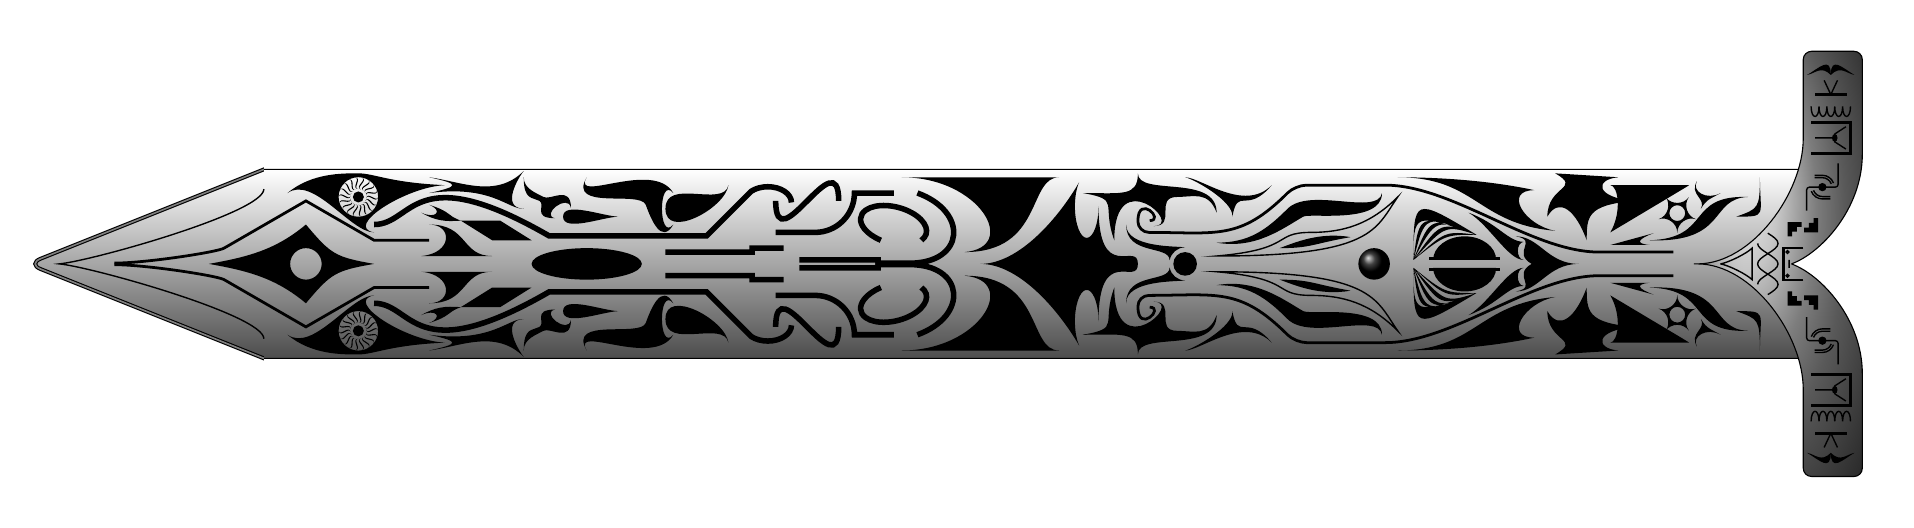
\begin{tikzpicture}[rotate=-90,every path/.style={line width=0.5pt,line join=miter,miter limit=25}]
\begin{scope}[every path/.style={}]
\clip (-3,1.5) rectangle +(6,-23.5);
\shadedraw[shading=axial,top color=white,bottom color=black!70] (-1.2,0.4) --++(0,-19.5) --++(1.2,-3)--++(1.2,3) --++(0,19.5)--(0,0)--cycle;
\shadedraw[shading=ball,ball color=black!30,rounded corners=3pt] 
	(0,0.3)..controls+(110:0.4) and +(0:0.8)..(-1.5,1.2)--(-2.7,1.2)--(-2.7,0.45)--(-1.7,0.45) .. controls +(0:0.8) and +(90:0.8) .. (0,-1)
	..controls+(90:0.8) and +(180:0.8)..(1.7,0.45)--(2.7,0.45)--(2.7,1.2)--(1.5,1.2)..controls+(180:0.8) and +(70:0.4)..(0,0.3);
\end{scope}
%
\begin{scope}[every path/.append style={xscale=\scal}]
\foreach \scal in {1,-1}{%
\draw[line width=0.8pt] (-0.2,0.45) --++(0,-0.25) -- ++(0.2,0);
\draw (-0.15,0.25)circle(0.5pt) (-0.05,0.27)--(0,0.27);
\draw (0,-0.2)--++(-0.2,0) .. controls +(-45:0.1) and +(100:0.1) .. (0,-0.6);
\draw (-0.39,0) sin ++(0.13,0.13) cos ++(0.13,-0.13) sin ++(0.13,-0.13)
	(-0.26,-0.13) cos ++(0.13,0.13) sin ++(0.13,0.13);
\fill (-0.35,0.25) -- ++(-0.18,0)--++(0,0.18)	--++(0.06,0)--++(0,-0.06)--++(0.06,0)--++(0,-0.06)--++(0.06,0)--++(0,-0.06)--cycle;
\fill[rotate=-90] 
	(-0.46,0.4) -- ++(-0.18,0)--++(0,0.18)--++(0.06,0)--++(0,-0.06)--++(0.06,0)--++(0,-0.06)--++(0.06,0)--++(0,-0.06)--cycle;
\draw[rounded corners=1pt](-0.675,0.493)--++(-0.3,0)--++(0,0.4)coordinate[pos=0.5](aa)--++(-0.3,0);
\fill (aa)circle(1.5pt);
\draw (aa)++(110:0.15)arc(110:180:0.15)--+(0,-0.1)
	(aa)++(-70:0.15)arc(-70:0:0.15) --+(0,0.1);
\draw (aa)++(110:0.12)arc(110:180:0.12)--+(0,-0.1)
	(aa)++(-70:0.12)arc(-70:0:0.12) --+(0,0.1);
\draw[line width=1.1pt] (-1.4,0.55)--++(0,0.5)--++(-0.4,0)--++(0,-0.5);
\fill (-1.6,0.85) ellipse(0.05cm and 1pt);
\draw (-1.6,0.85) --+(0,-0.25)
	+(-0.05,0)--
	+(0.05,0) --+(45:0.2)
	+(-0.05,0)--+(135:0.2);
\draw \foreach \y in {0.55,0.65,...,0.95}{%
		(-2,\y).. controls +(0:0.17) and +(0:0.17)..+(0,0.1)};
\draw[line width=1.2pt] (-2.15,0.6)--+(0,0.4);
\draw (-2.15,0.8) --+(155:0.2)
	(-2.15,0.8) --+(-155:0.2);
\fill (-2.4,0.8)..controls+(135:5pt) and +(-100:3pt)..(-2.4,1.1) .. controls +(-120:5pt) and +(180:7pt) .. (-2.4,0.8);
\fill (-2.4,0.8)..controls+(225:5pt) and +(100:3pt)..(-2.4,0.5) .. controls +(120:5pt) and +(180:7pt) .. (-2.4,0.8);
%
\draw[line width=1pt,rounded corners] (-0.15,-1.2) -- ++(0,-0.8)..controls+(-90:1) and +(90:1) .. (-1,-5)--
	++(0,-1).. controls+(-45:1) and +(90:1)..(-0.4,-8) .. controls +(180:0.5) and +(90:0.2) .. ++(-0.15,0.15);
\fill (-1.1,-0.1) ..controls +(0:0.5)  and +(90:0.4) .. (-0.6,-0.4)..controls +(110:0.3)  and +(-0.5:0.4) .. (-1.1,-0.1);
\fill (-0.85,-0.25)..controls+(-92:0.8) and +(92:0.8)..
	(-0.3,-1.5)..controls+(88:1) and +(-88:0.5)..(-0.85,-0.25);
\fill(-0.39,-1.45)..controls+(-70:0.2) and+(-95:0.2).. (-0.24,-1.5) -- (-0.24,-2)--cycle;
\fill (-0.9,-0.6) ..controls+(-61:0.2) and +(-29:0.15)..
	(-1.05,-0.9)..controls+(-31:0.2) and +(151:0.15)..
	(-0.7,-0.85)..controls+(149:0.15) and +(-59:0.15)..(-0.9,-0.6);
\path (-0.645,-1.15)coordinate(center)+(0:0.25)coordinate(p1) \foreach \an/\nom in  {72/p2,144/p3,216/p4,288/p5}  {+(\an:0.25)coordinate(\nom)};
\fill[even odd rule]
	(p1)..controls +(180:0.12) and +(108:0.12) ..(p5)
	..controls +(108:0.12) and +(36:0.12) ..(p4)
	..controls +(36:0.12) and +(324:0.12) ..(p3)
	..controls +(324:0.12) and +(252:0.12) ..(p2)
	..controls +(252:0.12) and +(180:0.12) ..(p1) 
	(center) circle(0.1);
\fill (-1,-1)--+(0,-1)..controls+(85:0.1) and +(150:0.3)..(-0.4,-2)..controls([xshift=0.15,yshift=-0.1]-1,-1)..(-1,-1);
\fill (-1.1,-1.9)..controls+(-85:0.3) and +(-95:0.5).. (-0.8,-1.7) ..controls+(-85:0.6) and +(180:0.3)..(-0.3,-2.3)
	..controls+(200:0.4) and+(150:0.3)..(-0.6,-2.8)..controls+(180:0.4) and +(60:0.4)..(-1.15,-2.7)--(-1.1,-1.9);
\fill (-0.42,-2.7)..controls+(-95:1) and +(90:1)..(-1.1,-4.7) arc (180:140:0.7cm and 2.7cm)
	..controls+(-90:0.4)and +(-100:0.4)..(-0.42,-2.7);
\fill (-0.28,-3.1)..controls+(-85:0.1) and +(-95:0.1)..(-0.05,-3.1) 
	..controls+(-90:0.2) and +(60:0.3).. (-0.65,-3.8)..controls+(70:0.4) and +(-90:0.2)..(-0.28,-3.1);
\fill (-0.05,-3.45) arc(90:270:0.3 and 0.4)--cycle;
\fill (-0.05,-3.4) rectangle +(-0.04,-0.9);
\fill[even odd rule] (-0.37,-3.7) .. controls +(-90:0.4)..(-0.05,-4.5)..controls+(180:0.8)..(-0.37,-3.7)
\foreach \an in{180,173,...,135}
{(-0.37,-3.7) .. controls +(-97:0.4)..(-0.05,-4.5)..controls +(\an:0.6)..(-0.37,-3.7)};
\draw (-0.85,-4.7)..controls+(-35:0.5) and+(90:2)..(-0.1,-7)..controls+(95:1) and +(-90:0.5) ..(-0.4,-5.8) ..controls+(90:0.4)and
		+(-45:0.5)..(-0.85,-4.7)--cycle;
\fill (-0.34,-5.3)..controls+(-80:0.5) and+(90:0.4).. (-0.2,-6.2)..controls+(110:0.2)and+(-100:0.4)..(-0.34,-5.3);
\fill(-0.9,-4.9) ..controls +(-10:0.3) and +(135:0.4).. 
	(-0.7,-6.1) ..controls+(-45:0.4) and +(90:0.4).. 
	(-0.27,-7)..controls+(80:0.5) and +(-60:0.3).. 
	(-0.6,-5.9)..controls+(120:0.1) and +(0:0.4)..(-0.9,-4.9);
\fill (-1,-6.3)..controls+(-40:0.5) and +(170:0.4)..(-0.6,-6.8)..controls+(175:0.2) and+(80:0.1)..(-1.1,-7.4)..controls+(90:0.2) and +(-45:0.5)..(-1,-6.3);
\fill (-0.65,-7) ..controls+(200:0.3) and +(90:0.2)..
	(-0.85,-7.5) .. controls +(-90:0.3) and +(90:0.3)..
	(-0.48,-7.8) .. controls+(90:0.4) and +(180:1)..
	(-0.3,-8.3)..controls+(200:0.5) and +(80:0.5)..
	(-0.9,-8.7) ..controls+(90:0.5) and +(0:0.3)..
	(-1.15,-8)..controls+(0:0.3) and +(180:0.5)..(-0.65,-7);
\fill (-0.21,-7.4) arc(180:260:0.2).. controls+(180:0.2) and +(0:0.4).. (-0.5,-8.15)..controls+(0:0.3) and +(-100:0.1)..(-0.21,-7.4);
\fill (-1.1,-9)..controls+(-90:0.4) and +(90:1)..
	(-0.15,-10.2)..controls+(95:0.7) and +(90:1)..
	(-1.1,-11)..controls+(90:0.2) and +(-90:0.2)..(-1.1,-9);
\draw[line width=2pt] (-0.9,-10.8)..controls+(70:0.7) and +(90:0.7)..(-0.00878735,-10.9)--++(0,-0.4) -| (-0.05,-12.3)
	(-0.9,-11.1)--++(0,-0.5)arc(90:0:0.5)--++(0,-0.5)
	(-0.2,-12.5)--++(0,-0.4) -| (-0.15,-14)
	(-0.78,-12.4)arc(90:225:0.2 and 0.3) -- ++(-45:0.8) -- ++(0,-2)..controls+(-120:2) and +(90:0.5)..(-0.5,-17.7)
	(-0.8,-11.8)..controls+(180:0.8)and+(0:0.8)..++(0,-0.8);
\draw[line width=2pt,yslant=0.5] (-0.3,-10.6)arc(40:320:0.25 and 0.4);
\draw[line width=1pt] (-0.3,-17)--(-0.3,-17.7) -- ++(240:1)--++(-60:1.2)..controls+(-60:0.1)and+(90:0.4)..(-0.01,-21);
\fill (-1,-13.2) ..controls+(-12:0.3) and +(180:0.4) .. (-0.7,-14) ..controls+(0:0.4) and +(-8:0.3)..(-1,-13.2);
\fill (-0.9,-13.9)..controls +(220:0.3) and +(-40:0.3)..(-0.5,-13.9)..controls +(-30:0.3) and +(20:0.2) ..
	(-0.75,-14.25) ..controls +(200:0.2) and +(-30:0.5)..(-1.1,-15)..controls+(-30:0.4) and +(210:0.5)..(-0.9,-13.9);
\fill (-0.6,-14.6)..controls+(-92:0.2) and +(180:0.2) .. (-0.6,-15.3)..controls +(0:0.2) and +(-88:0.2)..(-0.6,-14.6);
\fill (-0.7,-15.8)..controls+(-92.5:0.3)and+(-40:0.1)..
	(-1.18,-15.8)..controls+(-45:0.5)and+(82.5:0.4)..
	(-1.1,-17)..controls+(77.5:0.4)and+(102.5:0.4)..
	(-0.9,-17)..controls+(97.5:0.8)and+(-87.5:0.2)..
	(-0.7,-15.8);
\fill (-0.71,-15.2)..controls +(180:0.3) and +(60:0.1)..
	(-0.85,-15.55) ..controls +(-120:0.1) and +(0:0.15)..
	(-1.1,-15.8)..controls +(0:0.3) and +(-120:0.1)..
	(-0.8,-15.6)..controls +(60:0.1) and +(-90:0.3) ..
	(-0.58,-15.4) ..controls +(-100:0.2) and +(190:0.2)..(-0.71,-15.2);
\fill (-0.3,-15.7)--(-0.3,-16.2)--
	(-0.55,-16.6)..controls+(-85:0.2)and+(60:0.2)..
	(-0.65,-17.1)..controls+(65:0.2)and+(67.5:0.2)..
	(-0.75,-17)..controls+(72.5:0.3)and+(-110:0.2)..
	(-0.55,-16.6)--(-0.55,-16.1)--cycle;
\fill (-0.1,-17.1)..controls+(95:0.4)and+(90:0.3)..
	(-0.5,-17)..controls+(90:0.5)and+(-90:0.4)..
	(-0.1,-16.2)--cycle;
\fill (-1,-16.8) .. controls +(-87.5:0.5) and +(-100:0.4) ..
	(-0.4,-17.7)..controls+(-90:0.3) and +(125:0.4).. 
	(-0.9,-18.8)..controls+(130:0.4)and+(-90:0.2)..
	(-1.15,-17.9) ..controls+(90:0.2) and +(-92.5:0.7).. (-1,-16.8)
	(-0.85,-17.9) circle(0.251);
\foreach \an in {0,20,...,340}{%
	\pgfmathadd{\an}{10}\let\x\pgfmathresult
\path (-0.85,-17.9) +(\an:0.1)coordinate(sc1\an);
\path (-0.85,-17.9)+(\x:0.25)coordinate(sc2\an);
}
\foreach \an in {-90,-70,...,250}{%
	\pgfmathadd{180}{\an}\let\x\pgfmathresult
	\pgfmathadd{90}{\an}\let\y\pgfmathresult
\fill	(sc2\y)..controls +(\an:0.08)and +(\x:0.1).. (sc1\y)..controls+(\x:0.08)and+(\an:0.1)..(sc2\y);}
\fill (-0.85,-17.9) circle(0.07);
}
\end{scope}
\fill (0,-2.4) ..controls+(-90:0.4) and +(90:0.3) .. 
	(-0.35,-3.2)..controls+(80:0.3) and +(240:0.3)..
	(0,-3)..controls+(-60:0.3) and +(100:0.3)..
	(0.35,-3.2)..controls +(90:0.3) and +(-90:0.4) .. (0,-2.4);
\shade[shading=ball,ball color=black] (0,-5)circle(0.2);
\fill (0,-7.4) circle(0.15);
\fill (0,-8) ..controls +(180:0.3) and +(0:1).. (-0.73,-8.5) arc(90:-140:0.4 and 0.15)coordinate(ar)..controls +(-30:0.5) and +(90:0.5) ..
	(0,-10)..controls +(90:0.5) and +(-150:0.5) ..([xscale=-1]ar) arc(-40:-270:0.4 and 0.15)..controls +(180:1) and +(0:0.3) .. (0,-8);
\fill (0,-15) ellipse(0.2 and 0.7);
\draw (-0.95,-19.1)..controls+(0:0.3) and +(95:0.4) ..(0,-21.7)..controls+(85:0.4) and +(180:0.3)..(0.95,-19.1);
\fill[even odd rule] (0,-17.7)..controls+(260:0.5)and+(40:0.5)..
			++(240:1)coordinate(tmp)..controls+(-50:0.5)and+(100:0.5)..
			(0,-19.8)..controls+(80:0.5)and+(230:0.5)..
			([xscale=-1]tmp) ..controls+(140:0.5)and+(-80:0.5)..(0,-17.7)
(0,-18.566)circle(0.2);
\begin{scope}[every path/.style={}]
\clip (-1.4,-19.1) rectangle +(3,-3);
\draw[double=black!50,rounded corners=5pt] (-1.2,-19.1)+(-1.2,3)--++(1.2,-3)--++(2.4,6);
\end{scope}
\end{tikzpicture}

\end{document}
